\documentclass[1p]{elsarticle_modified}
%\bibliographystyle{elsarticle-num}

%\usepackage[colorlinks]{hyperref}
%\usepackage{abbrmath_seonhwa} %\Abb, \Ascr, \Acal ,\Abf, \Afrak
\usepackage{amsfonts}
\usepackage{amssymb}
\usepackage{amsmath}
\usepackage{amsthm}
\usepackage{scalefnt}
\usepackage{amsbsy}
\usepackage{kotex}
\usepackage{caption}
\usepackage{subfig}
\usepackage{color}
\usepackage{graphicx}
\usepackage{xcolor} %% white, black, red, green, blue, cyan, magenta, yellow
\usepackage{float}
\usepackage{setspace}
\usepackage{hyperref}

\usepackage{tikz}
\usetikzlibrary{arrows}

\usepackage{multirow}
\usepackage{array} % fixed length table
\usepackage{hhline}

%%%%%%%%%%%%%%%%%%%%%
\makeatletter
\renewcommand*\env@matrix[1][\arraystretch]{%
	\edef\arraystretch{#1}%
	\hskip -\arraycolsep
	\let\@ifnextchar\new@ifnextchar
	\array{*\c@MaxMatrixCols c}}
\makeatother %https://tex.stackexchange.com/questions/14071/how-can-i-increase-the-line-spacing-in-a-matrix
%%%%%%%%%%%%%%%

\usepackage[normalem]{ulem}

\newcommand{\msout}[1]{\ifmmode\text{\sout{\ensuremath{#1}}}\else\sout{#1}\fi}
%SOURCE: \msout is \stkout macro in https://tex.stackexchange.com/questions/20609/strikeout-in-math-mode

\newcommand{\cancel}[1]{
	\ifmmode
	{\color{red}\msout{#1}}
	\else
	{\color{red}\sout{#1}}
	\fi
}

\newcommand{\add}[1]{
	{\color{blue}\uwave{#1}}
}

\newcommand{\replace}[2]{
	\ifmmode
	{\color{red}\msout{#1}}{\color{blue}\uwave{#2}}
	\else
	{\color{red}\sout{#1}}{\color{blue}\uwave{#2}}
	\fi
}

\newcommand{\Sol}{\mathcal{S}} %segment
\newcommand{\D}{D} %diagram
\newcommand{\A}{\mathcal{A}} %arc


%%%%%%%%%%%%%%%%%%%%%%%%%%%%%5 test

\def\sl{\operatorname{\textup{SL}}(2,\Cbb)}
\def\psl{\operatorname{\textup{PSL}}(2,\Cbb)}
\def\quan{\mkern 1mu \triangleright \mkern 1mu}

\theoremstyle{definition}
\newtheorem{thm}{Theorem}[section]
\newtheorem{prop}[thm]{Proposition}
\newtheorem{lem}[thm]{Lemma}
\newtheorem{ques}[thm]{Question}
\newtheorem{cor}[thm]{Corollary}
\newtheorem{defn}[thm]{Definition}
\newtheorem{exam}[thm]{Example}
\newtheorem{rmk}[thm]{Remark}
\newtheorem{alg}[thm]{Algorithm}

\newcommand{\I}{\sqrt{-1}}
\begin{document}

%\begin{frontmatter}
%
%\title{Boundary parabolic representations of knots up to 8 crossings}
%
%%% Group authors per affiliation:
%\author{Yunhi Cho} 
%\address{Department of Mathematics, University of Seoul, Seoul, Korea}
%\ead{yhcho@uos.ac.kr}
%
%
%\author{Seonhwa Kim} %\fnref{s_kim}}
%\address{Center for Geometry and Physics, Institute for Basic Science, Pohang, 37673, Korea}
%\ead{ryeona17@ibs.re.kr}
%
%\author{Hyuk Kim}
%\address{Department of Mathematical Sciences, Seoul National University, Seoul 08826, Korea}
%\ead{hyukkim@snu.ac.kr}
%
%\author{Seokbeom Yoon}
%\address{Department of Mathematical Sciences, Seoul National University, Seoul, 08826,  Korea}
%\ead{sbyoon15@snu.ac.kr}
%
%\begin{abstract}
%We find all boundary parabolic representation of knots up to 8 crossings.
%
%\end{abstract}
%\begin{keyword}
%    \MSC[2010] 57M25 
%\end{keyword}
%
%\end{frontmatter}

%\linenumbers
%\tableofcontents
%
\newcommand\colored[1]{\textcolor{white}{\rule[-0.35ex]{0.8em}{1.4ex}}\kern-0.8em\color{red} #1}%
%\newcommand\colored[1]{\textcolor{white}{ #1}\kern-2.17ex	\textcolor{white}{ #1}\kern-1.81ex	\textcolor{white}{ #1}\kern-2.15ex\color{red}#1	}

{\Large $\underline{11a_{200}~(K11a_{200})}$}

\setlength{\tabcolsep}{10pt}
\renewcommand{\arraystretch}{1.6}
\vspace{1cm}\begin{tabular}{m{100pt}>{\centering\arraybackslash}m{274pt}}
\multirow{5}{120pt}{
	\centering
	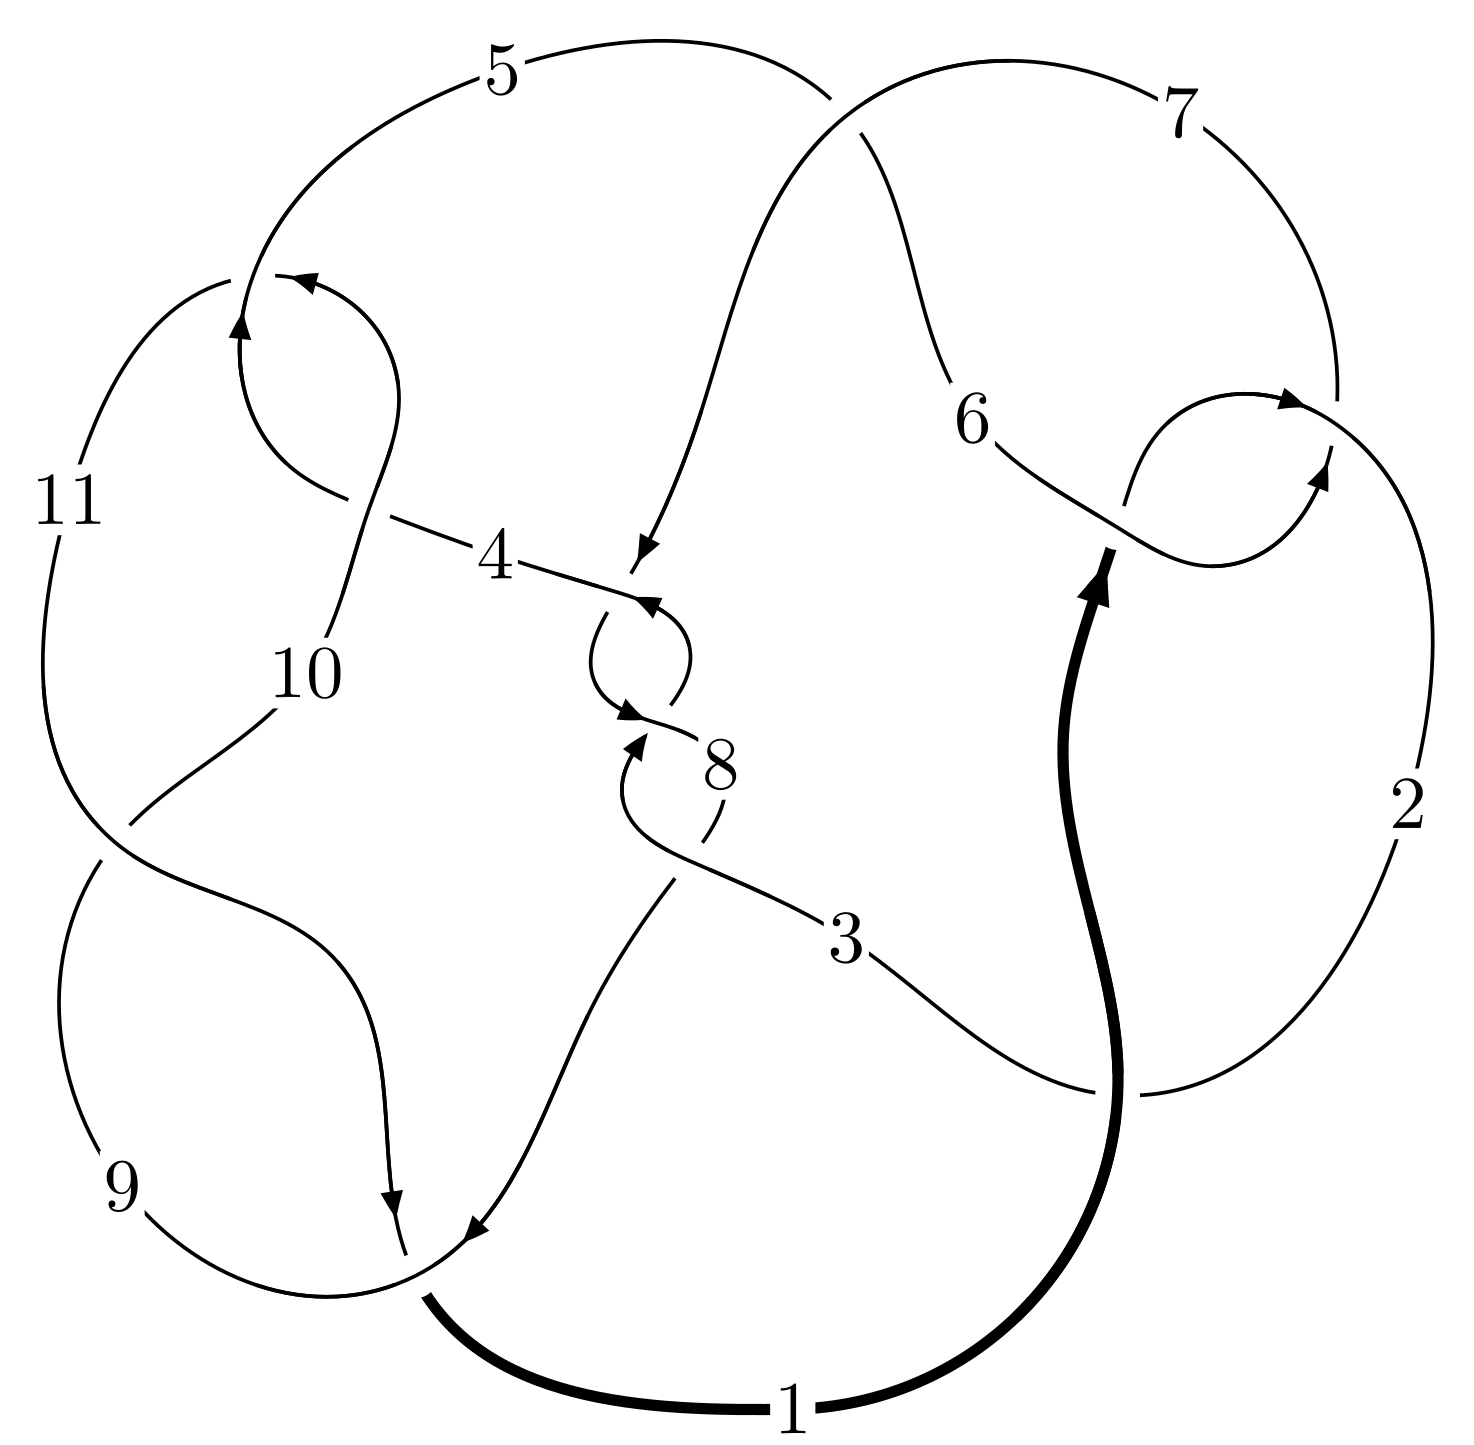
\includegraphics[width=112pt]{../../../GIT/diagram.site/Diagrams/png/449_11a_200.png}\\
\ \ \ A knot diagram\footnotemark}&
\allowdisplaybreaks
\textbf{Linearized knot diagam} \\
\cline{2-2}
 &
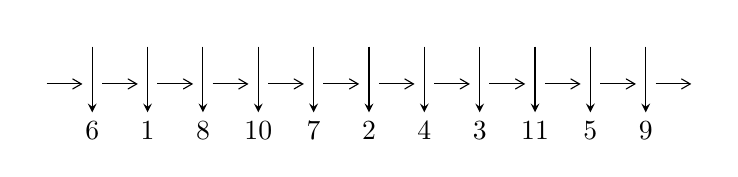
\begin{tikzpicture}[x=20pt, y=17pt]
	% nodes
	\node (C0) at (0, 0) {};
	\node (C1) at (1, 0) {};
	\node (C1U) at (1, +1) {};
	\node (C1D) at (1, -1) {6};

	\node (C2) at (2, 0) {};
	\node (C2U) at (2, +1) {};
	\node (C2D) at (2, -1) {1};

	\node (C3) at (3, 0) {};
	\node (C3U) at (3, +1) {};
	\node (C3D) at (3, -1) {8};

	\node (C4) at (4, 0) {};
	\node (C4U) at (4, +1) {};
	\node (C4D) at (4, -1) {10};

	\node (C5) at (5, 0) {};
	\node (C5U) at (5, +1) {};
	\node (C5D) at (5, -1) {7};

	\node (C6) at (6, 0) {};
	\node (C6U) at (6, +1) {};
	\node (C6D) at (6, -1) {2};

	\node (C7) at (7, 0) {};
	\node (C7U) at (7, +1) {};
	\node (C7D) at (7, -1) {4};

	\node (C8) at (8, 0) {};
	\node (C8U) at (8, +1) {};
	\node (C8D) at (8, -1) {3};

	\node (C9) at (9, 0) {};
	\node (C9U) at (9, +1) {};
	\node (C9D) at (9, -1) {11};

	\node (C10) at (10, 0) {};
	\node (C10U) at (10, +1) {};
	\node (C10D) at (10, -1) {5};

	\node (C11) at (11, 0) {};
	\node (C11U) at (11, +1) {};
	\node (C11D) at (11, -1) {9};
	\node (C12) at (12, 0) {};

	% arrows
	\draw[->,>={angle 60}]
	(C0) edge (C1) (C1) edge (C2) (C2) edge (C3) (C3) edge (C4) (C4) edge (C5) (C5) edge (C6) (C6) edge (C7) (C7) edge (C8) (C8) edge (C9) (C9) edge (C10) (C10) edge (C11) (C11) edge (C12) ;	\draw[->,>=stealth]
	(C1U) edge (C1D) (C2U) edge (C2D) (C3U) edge (C3D) (C4U) edge (C4D) (C5U) edge (C5D) (C6U) edge (C6D) (C7U) edge (C7D) (C8U) edge (C8D) (C9U) edge (C9D) (C10U) edge (C10D) (C11U) edge (C11D) ;
	\end{tikzpicture} \\
\hhline{~~} \\& 
\textbf{Solving Sequence} \\ \cline{2-2} 
 &
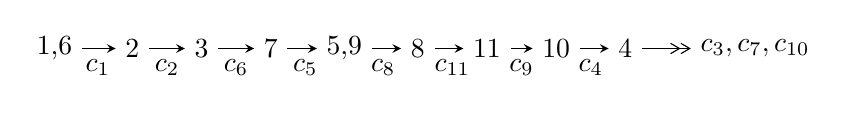
\begin{tikzpicture}[x=25pt, y=7pt]
	% node
	\node (A0) at (-1/8, 0) {1,6};
	\node (A1) at (1, 0) {2};
	\node (A2) at (2, 0) {3};
	\node (A3) at (3, 0) {7};
	\node (A4) at (65/16, 0) {5,9};
	\node (A5) at (41/8, 0) {8};
	\node (A6) at (49/8, 0) {11};
	\node (A7) at (57/8, 0) {10};
	\node (A8) at (65/8, 0) {4};
	\node (C1) at (1/2, -1) {$c_{1}$};
	\node (C2) at (3/2, -1) {$c_{2}$};
	\node (C3) at (5/2, -1) {$c_{6}$};
	\node (C4) at (7/2, -1) {$c_{5}$};
	\node (C5) at (37/8, -1) {$c_{8}$};
	\node (C6) at (45/8, -1) {$c_{11}$};
	\node (C7) at (53/8, -1) {$c_{9}$};
	\node (C8) at (61/8, -1) {$c_{4}$};
	\node (A9) at (10, 0) {$c_{3},c_{7},c_{10}$};

	% edge
	\draw[->,>=stealth]	
	(A0) edge (A1) (A1) edge (A2) (A2) edge (A3) (A3) edge (A4) (A4) edge (A5) (A5) edge (A6) (A6) edge (A7) (A7) edge (A8) ;
	\draw[->>,>={angle 60}]	
	(A8) edge (A9);
\end{tikzpicture} \\ 

\end{tabular} \\

\footnotetext{
The image of knot diagram is generated by the software ``\textbf{Draw programme}" developed by Andrew Bartholomew(\url{http://www.layer8.co.uk/maths/draw/index.htm\#Running-draw}), where we modified some parts for our purpose(\url{https://github.com/CATsTAILs/LinksPainter}).
}\phantom \\ \newline 
\centering \textbf{Ideals for irreducible components\footnotemark of $X_{\text{par}}$} 
 
\begin{align*}
I^u_{1}&=\langle 
u^2+b,\;- u^{13}+u^{11}+u^{10}-4 u^9+3 u^7+4 u^6-4 u^5-2 u^4+3 u^3+3 u^2+2 a+u-3,\\
\phantom{I^u_{1}}&\phantom{= \langle  }u^{14}-2 u^{12}+6 u^{10}- u^9-8 u^8+u^7+10 u^6-2 u^5-9 u^4+u^3+4 u^2+u-1\rangle \\
I^u_{2}&=\langle 
11044796022984 u^{35}+15849610659410 u^{34}+\cdots+5213417579383 b-19244867589607,\\
\phantom{I^u_{2}}&\phantom{= \langle  }-20597520331605 u^{35}-27230487651401 u^{34}+\cdots+5213417579383 a+39323690068543,\\
\phantom{I^u_{2}}&\phantom{= \langle  }u^{36}+u^{35}+\cdots-2 u+1\rangle \\
I^u_{3}&=\langle 
u^2+b,\;- u^2+a- u+1,\;u^4- u^2+1\rangle \\
I^u_{4}&=\langle 
- u^2+b+1,\;a- u-1,\;u^4- u^2+1\rangle \\
\\
\end{align*}
\raggedright * 4 irreducible components of $\dim_{\mathbb{C}}=0$, with total 58 representations.\\
\footnotetext{All coefficients of polynomials are rational numbers. But the coefficients are sometimes approximated in decimal forms when there is not enough margin.}
\newpage
\renewcommand{\arraystretch}{1}
\centering \section*{I. $I^u_{1}= \langle u^2+b,\;- u^{13}+u^{11}+\cdots+2 a-3,\;u^{14}-2 u^{12}+\cdots+u-1 \rangle$}
\flushleft \textbf{(i) Arc colorings}\\
\begin{tabular}{m{7pt} m{180pt} m{7pt} m{180pt} }
\flushright $a_{1}=$&$\begin{pmatrix}1\\0\end{pmatrix}$ \\
\flushright $a_{6}=$&$\begin{pmatrix}0\\u\end{pmatrix}$ \\
\flushright $a_{2}=$&$\begin{pmatrix}1\\u^2\end{pmatrix}$ \\
\flushright $a_{3}=$&$\begin{pmatrix}- u^2+1\\u^2\end{pmatrix}$ \\
\flushright $a_{7}=$&$\begin{pmatrix}- u\\- u^3+u\end{pmatrix}$ \\
\flushright $a_{5}=$&$\begin{pmatrix}u^3\\u^5- u^3+u\end{pmatrix}$ \\
\flushright $a_{9}=$&$\begin{pmatrix}\frac{1}{2} u^{13}-\frac{1}{2} u^{11}+\cdots-\frac{1}{2} u+\frac{3}{2}\\- u^2\end{pmatrix}$ \\
\flushright $a_{8}=$&$\begin{pmatrix}- u^6+u^4-2 u^2+1\\\frac{1}{2} u^{12}+\frac{1}{2} u^{11}+\cdots- u+\frac{1}{2}\end{pmatrix}$ \\
\flushright $a_{11}=$&$\begin{pmatrix}\frac{1}{2} u^{13}-\frac{1}{2} u^{12}+\cdots+\frac{1}{2} u+1\\- u^4\end{pmatrix}$ \\
\flushright $a_{10}=$&$\begin{pmatrix}\frac{1}{2} u^{13}-\frac{1}{2} u^{12}+\cdots+\frac{1}{2} u+1\\- u^6- u^2\end{pmatrix}$ \\
\flushright $a_{4}=$&$\begin{pmatrix}-\frac{1}{2} u^{13}+\frac{1}{2} u^{11}+\cdots+\frac{1}{2} u+\frac{1}{2}\\- u^7+u^5-2 u^3+u\end{pmatrix}$\\ \flushright $a_{4}=$&$\begin{pmatrix}-\frac{1}{2} u^{13}+\frac{1}{2} u^{11}+\cdots+\frac{1}{2} u+\frac{1}{2}\\- u^7+u^5-2 u^3+u\end{pmatrix}$\\&\end{tabular}
\flushleft \textbf{(ii) Obstruction class $= -1$}\\~\\
\flushleft \textbf{(iii) Cusp Shapes $= u^{13}+u^{11}+u^{10}+2 u^9-4 u^8+7 u^7+4 u^6-4 u^5-10 u^4+11 u^3+5 u^2-9 u-13$}\\~\\
\newpage\renewcommand{\arraystretch}{1}
\flushleft \textbf{(iv) u-Polynomials at the component}\newline \\
\begin{tabular}{m{50pt}|m{274pt}}
Crossings & \hspace{64pt}u-Polynomials at each crossing \\
\hline $$\begin{aligned}c_{1},c_{4},c_{6}\\c_{10}\end{aligned}$$&$\begin{aligned}
&u^{14}-2 u^{12}+6 u^{10}+u^9-8 u^8- u^7+10 u^6+2 u^5-9 u^4- u^3+4 u^2- u-1
\end{aligned}$\\
\hline $$\begin{aligned}c_{2},c_{5},c_{9}\\c_{11}\end{aligned}$$&$\begin{aligned}
&u^{14}+4 u^{13}+\cdots+9 u+1
\end{aligned}$\\
\hline $$\begin{aligned}c_{3},c_{7},c_{8}\end{aligned}$$&$\begin{aligned}
&u^{14}-5 u^{13}+\cdots+8 u-4
\end{aligned}$\\
\hline
\end{tabular}\\~\\
\newpage\renewcommand{\arraystretch}{1}
\flushleft \textbf{(v) Riley Polynomials at the component}\newline \\
\begin{tabular}{m{50pt}|m{274pt}}
Crossings & \hspace{64pt}Riley Polynomials at each crossing \\
\hline $$\begin{aligned}c_{1},c_{4},c_{6}\\c_{10}\end{aligned}$$&$\begin{aligned}
&y^{14}-4 y^{13}+\cdots-9 y+1
\end{aligned}$\\
\hline $$\begin{aligned}c_{2},c_{5},c_{9}\\c_{11}\end{aligned}$$&$\begin{aligned}
&y^{14}+16 y^{13}+\cdots-17 y+1
\end{aligned}$\\
\hline $$\begin{aligned}c_{3},c_{7},c_{8}\end{aligned}$$&$\begin{aligned}
&y^{14}+13 y^{13}+\cdots-136 y+16
\end{aligned}$\\
\hline
\end{tabular}\\~\\
\newpage\flushleft \textbf{(vi) Complex Volumes and Cusp Shapes}
$$\begin{array}{c|c|c}  
\text{Solutions to }I^u_{1}& \I (\text{vol} + \sqrt{-1}CS) & \text{Cusp shape}\\
 \hline 
\begin{aligned}
u &= -0.950366\phantom{ +0.000000I} \\
a &= -0.787840\phantom{ +0.000000I} \\
b &= -0.903195\phantom{ +0.000000I}\end{aligned}
 & -4.35310\phantom{ +0.000000I} & -20.7960\phantom{ +0.000000I} \\ \hline\begin{aligned}
u &= \phantom{-}0.934140 + 0.165940 I \\
a &= -0.833929 - 0.848131 I \\
b &= -0.845081 - 0.310022 I\end{aligned}
 & -0.76895 - 3.05854 I & -15.2345 + 4.4220 I \\ \hline\begin{aligned}
u &= \phantom{-}0.934140 - 0.165940 I \\
a &= -0.833929 + 0.848131 I \\
b &= -0.845081 + 0.310022 I\end{aligned}
 & -0.76895 + 3.05854 I & -15.2345 - 4.4220 I \\ \hline\begin{aligned}
u &= -0.861511 + 0.818074 I \\
a &= -0.43826 - 2.03212 I \\
b &= -0.072957 + 1.409560 I\end{aligned}
 & \phantom{-}6.31411 + 3.07801 I & -6.07433 - 2.66063 I \\ \hline\begin{aligned}
u &= -0.861511 - 0.818074 I \\
a &= -0.43826 + 2.03212 I \\
b &= -0.072957 - 1.409560 I\end{aligned}
 & \phantom{-}6.31411 - 3.07801 I & -6.07433 + 2.66063 I \\ \hline\begin{aligned}
u &= \phantom{-}0.771614 + 0.940827 I \\
a &= -0.178207 + 1.387930 I \\
b &= \phantom{-}0.28977 - 1.45191 I\end{aligned}
 & \phantom{-}14.2923 + 0.8767 I & -3.65848 + 1.44035 I \\ \hline\begin{aligned}
u &= \phantom{-}0.771614 - 0.940827 I \\
a &= -0.178207 - 1.387930 I \\
b &= \phantom{-}0.28977 + 1.45191 I\end{aligned}
 & \phantom{-}14.2923 - 0.8767 I & -3.65848 - 1.44035 I \\ \hline\begin{aligned}
u &= \phantom{-}0.965155 + 0.787055 I \\
a &= -1.13614 + 2.04636 I \\
b &= -0.31207 - 1.51926 I\end{aligned}
 & \phantom{-}5.64578 - 9.04247 I & -7.75570 + 7.54934 I \\ \hline\begin{aligned}
u &= \phantom{-}0.965155 - 0.787055 I \\
a &= -1.13614 - 2.04636 I \\
b &= -0.31207 + 1.51926 I\end{aligned}
 & \phantom{-}5.64578 + 9.04247 I & -7.75570 - 7.54934 I \\ \hline\begin{aligned}
u &= -0.499772 + 0.464713 I \\
a &= \phantom{-}1.46491 - 0.18431 I \\
b &= -0.033814 + 0.464501 I\end{aligned}
 & \phantom{-}2.42034 + 2.01219 I & -5.03531 - 3.18410 I\\
 \hline 
 \end{array}$$\newpage$$\begin{array}{c|c|c}  
\text{Solutions to }I^u_{1}& \I (\text{vol} + \sqrt{-1}CS) & \text{Cusp shape}\\
 \hline 
\begin{aligned}
u &= -0.499772 - 0.464713 I \\
a &= \phantom{-}1.46491 + 0.18431 I \\
b &= -0.033814 - 0.464501 I\end{aligned}
 & \phantom{-}2.42034 - 2.01219 I & -5.03531 + 3.18410 I \\ \hline\begin{aligned}
u &= -1.055500 + 0.798468 I \\
a &= -1.43912 - 1.62917 I \\
b &= -0.47652 + 1.68556 I\end{aligned}
 & \phantom{-}12.4304 + 13.7591 I & -6.11753 - 7.81595 I \\ \hline\begin{aligned}
u &= -1.055500 - 0.798468 I \\
a &= -1.43912 + 1.62917 I \\
b &= -0.47652 - 1.68556 I\end{aligned}
 & \phantom{-}12.4304 - 13.7591 I & -6.11753 + 7.81595 I \\ \hline\begin{aligned}
u &= \phantom{-}0.442106\phantom{ +0.000000I} \\
a &= \phantom{-}0.909335\phantom{ +0.000000I} \\
b &= -0.195458\phantom{ +0.000000I}\end{aligned}
 & -0.647887\phantom{ +0.000000I} & -15.4520\phantom{ +0.000000I}\\
 \hline 
 \end{array}$$\newpage\newpage\renewcommand{\arraystretch}{1}
\centering \section*{II. $I^u_{2}= \langle 1.10\times10^{13} u^{35}+1.58\times10^{13} u^{34}+\cdots+5.21\times10^{12} b-1.92\times10^{13},\;-2.06\times10^{13} u^{35}-2.72\times10^{13} u^{34}+\cdots+5.21\times10^{12} a+3.93\times10^{13},\;u^{36}+u^{35}+\cdots-2 u+1 \rangle$}
\flushleft \textbf{(i) Arc colorings}\\
\begin{tabular}{m{7pt} m{180pt} m{7pt} m{180pt} }
\flushright $a_{1}=$&$\begin{pmatrix}1\\0\end{pmatrix}$ \\
\flushright $a_{6}=$&$\begin{pmatrix}0\\u\end{pmatrix}$ \\
\flushright $a_{2}=$&$\begin{pmatrix}1\\u^2\end{pmatrix}$ \\
\flushright $a_{3}=$&$\begin{pmatrix}- u^2+1\\u^2\end{pmatrix}$ \\
\flushright $a_{7}=$&$\begin{pmatrix}- u\\- u^3+u\end{pmatrix}$ \\
\flushright $a_{5}=$&$\begin{pmatrix}u^3\\u^5- u^3+u\end{pmatrix}$ \\
\flushright $a_{9}=$&$\begin{pmatrix}3.95087 u^{35}+5.22315 u^{34}+\cdots+0.910129 u-7.54279\\-2.11853 u^{35}-3.04016 u^{34}+\cdots-2.06187 u+3.69141\end{pmatrix}$ \\
\flushright $a_{8}=$&$\begin{pmatrix}2.27927 u^{35}+2.86643 u^{34}+\cdots-0.0438616 u-4.50374\\-2.47612 u^{35}-3.71564 u^{34}+\cdots-2.03874 u+4.69444\end{pmatrix}$ \\
\flushright $a_{11}=$&$\begin{pmatrix}-2.30128 u^{35}-3.92404 u^{34}+\cdots+1.16386 u+3.30524\\-2.34203 u^{35}-3.45720 u^{34}+\cdots-1.18510 u+5.47128\end{pmatrix}$ \\
\flushright $a_{10}=$&$\begin{pmatrix}-1.79396 u^{35}-3.71712 u^{34}+\cdots+0.968286 u+3.13328\\-1.97576 u^{35}-2.57126 u^{34}+\cdots-0.845464 u+4.81490\end{pmatrix}$ \\
\flushright $a_{4}=$&$\begin{pmatrix}4.69444 u^{35}+7.17055 u^{34}+\cdots-0.960342 u-7.35013\\0.587159 u^{35}+0.875255 u^{34}+\cdots+0.0548089 u-2.27927\end{pmatrix}$\\ \flushright $a_{4}=$&$\begin{pmatrix}4.69444 u^{35}+7.17055 u^{34}+\cdots-0.960342 u-7.35013\\0.587159 u^{35}+0.875255 u^{34}+\cdots+0.0548089 u-2.27927\end{pmatrix}$\\&\end{tabular}
\flushleft \textbf{(ii) Obstruction class $= -1$}\\~\\
\flushleft \textbf{(iii) Cusp Shapes $= \frac{23301194605224}{5213417579383} u^{35}+\frac{35979605140824}{5213417579383} u^{34}+\cdots+\frac{21746030582642}{5213417579383} u-\frac{88939694002132}{5213417579383}$}\\~\\
\newpage\renewcommand{\arraystretch}{1}
\flushleft \textbf{(iv) u-Polynomials at the component}\newline \\
\begin{tabular}{m{50pt}|m{274pt}}
Crossings & \hspace{64pt}u-Polynomials at each crossing \\
\hline $$\begin{aligned}c_{1},c_{4},c_{6}\\c_{10}\end{aligned}$$&$\begin{aligned}
&u^{36}- u^{35}+\cdots+2 u+1
\end{aligned}$\\
\hline $$\begin{aligned}c_{2},c_{5},c_{9}\\c_{11}\end{aligned}$$&$\begin{aligned}
&u^{36}+11 u^{35}+\cdots+2 u+1
\end{aligned}$\\
\hline $$\begin{aligned}c_{3},c_{7},c_{8}\end{aligned}$$&$\begin{aligned}
&(u^{18}+2 u^{17}+\cdots+4 u+1)^{2}
\end{aligned}$\\
\hline
\end{tabular}\\~\\
\newpage\renewcommand{\arraystretch}{1}
\flushleft \textbf{(v) Riley Polynomials at the component}\newline \\
\begin{tabular}{m{50pt}|m{274pt}}
Crossings & \hspace{64pt}Riley Polynomials at each crossing \\
\hline $$\begin{aligned}c_{1},c_{4},c_{6}\\c_{10}\end{aligned}$$&$\begin{aligned}
&y^{36}-11 y^{35}+\cdots-2 y+1
\end{aligned}$\\
\hline $$\begin{aligned}c_{2},c_{5},c_{9}\\c_{11}\end{aligned}$$&$\begin{aligned}
&y^{36}+29 y^{35}+\cdots-86 y+1
\end{aligned}$\\
\hline $$\begin{aligned}c_{3},c_{7},c_{8}\end{aligned}$$&$\begin{aligned}
&(y^{18}+20 y^{17}+\cdots-6 y+1)^{2}
\end{aligned}$\\
\hline
\end{tabular}\\~\\
\newpage\flushleft \textbf{(vi) Complex Volumes and Cusp Shapes}
$$\begin{array}{c|c|c}  
\text{Solutions to }I^u_{2}& \I (\text{vol} + \sqrt{-1}CS) & \text{Cusp shape}\\
 \hline 
\begin{aligned}
u &= -0.812169 + 0.607179 I \\
a &= \phantom{-}0.671292 + 0.171361 I \\
b &= \phantom{-}0.144113 - 0.052398 I\end{aligned}
 & \phantom{-}1.69238 + 2.34050 I & -6.11304 - 4.51747 I \\ \hline\begin{aligned}
u &= -0.812169 - 0.607179 I \\
a &= \phantom{-}0.671292 - 0.171361 I \\
b &= \phantom{-}0.144113 + 0.052398 I\end{aligned}
 & \phantom{-}1.69238 - 2.34050 I & -6.11304 + 4.51747 I \\ \hline\begin{aligned}
u &= -0.946964 + 0.251366 I \\
a &= -1.156670 - 0.366820 I \\
b &= -0.466192 + 1.168730 I\end{aligned}
 & -0.82103 + 4.83091 I & -14.6707 - 7.5484 I \\ \hline\begin{aligned}
u &= -0.946964 - 0.251366 I \\
a &= -1.156670 + 0.366820 I \\
b &= -0.466192 - 1.168730 I\end{aligned}
 & -0.82103 - 4.83091 I & -14.6707 + 7.5484 I \\ \hline\begin{aligned}
u &= \phantom{-}0.730851 + 0.539733 I \\
a &= \phantom{-}0.924619 - 0.162335 I \\
b &= -0.543811 + 0.535375 I\end{aligned}
 & -0.218413 + 0.059150 I & -13.30450 - 1.20964 I \\ \hline\begin{aligned}
u &= \phantom{-}0.730851 - 0.539733 I \\
a &= \phantom{-}0.924619 + 0.162335 I \\
b &= -0.543811 - 0.535375 I\end{aligned}
 & -0.218413 - 0.059150 I & -13.30450 + 1.20964 I \\ \hline\begin{aligned}
u &= -0.942145 + 0.554752 I \\
a &= \phantom{-}0.794075 - 0.773298 I \\
b &= -0.251878 + 0.053017 I\end{aligned}
 & \phantom{-}1.36390 + 2.08554 I & -9.56168 - 2.20642 I \\ \hline\begin{aligned}
u &= -0.942145 - 0.554752 I \\
a &= \phantom{-}0.794075 + 0.773298 I \\
b &= -0.251878 - 0.053017 I\end{aligned}
 & \phantom{-}1.36390 - 2.08554 I & -9.56168 + 2.20642 I \\ \hline\begin{aligned}
u &= -0.040087 + 0.897653 I \\
a &= \phantom{-}0.20998 - 1.45458 I \\
b &= -0.11524 + 1.50569 I\end{aligned}
 & \phantom{-}9.19677 + 3.10798 I & -3.50971 - 2.64457 I \\ \hline\begin{aligned}
u &= -0.040087 - 0.897653 I \\
a &= \phantom{-}0.20998 + 1.45458 I \\
b &= -0.11524 - 1.50569 I\end{aligned}
 & \phantom{-}9.19677 - 3.10798 I & -3.50971 + 2.64457 I\\
 \hline 
 \end{array}$$\newpage$$\begin{array}{c|c|c}  
\text{Solutions to }I^u_{2}& \I (\text{vol} + \sqrt{-1}CS) & \text{Cusp shape}\\
 \hline 
\begin{aligned}
u &= \phantom{-}0.928565 + 0.629318 I \\
a &= -0.112955 + 1.243650 I \\
b &= -0.833557 - 0.476070 I\end{aligned}
 & -0.82103 - 4.83091 I & -14.6707 + 7.5484 I \\ \hline\begin{aligned}
u &= \phantom{-}0.928565 - 0.629318 I \\
a &= -0.112955 - 1.243650 I \\
b &= -0.833557 + 0.476070 I\end{aligned}
 & -0.82103 + 4.83091 I & -14.6707 - 7.5484 I \\ \hline\begin{aligned}
u &= \phantom{-}0.808373 + 0.331144 I \\
a &= \phantom{-}1.193410 - 0.008565 I \\
b &= -0.242832 + 0.788929 I\end{aligned}
 & -0.218413 - 0.059150 I & -13.30450 + 1.20964 I \\ \hline\begin{aligned}
u &= \phantom{-}0.808373 - 0.331144 I \\
a &= \phantom{-}1.193410 + 0.008565 I \\
b &= -0.242832 - 0.788929 I\end{aligned}
 & -0.218413 + 0.059150 I & -13.30450 - 1.20964 I \\ \hline\begin{aligned}
u &= -0.823976 + 0.805806 I \\
a &= \phantom{-}0.742818 - 0.074215 I \\
b &= -1.25591 - 0.81116 I\end{aligned}
 & \phantom{-}5.35610 - 1.19422 I & -7.28872 + 0.77166 I \\ \hline\begin{aligned}
u &= -0.823976 - 0.805806 I \\
a &= \phantom{-}0.742818 + 0.074215 I \\
b &= -1.25591 + 0.81116 I\end{aligned}
 & \phantom{-}5.35610 + 1.19422 I & -7.28872 - 0.77166 I \\ \hline\begin{aligned}
u &= \phantom{-}0.812050 + 0.836206 I \\
a &= \phantom{-}0.83079 - 1.99521 I \\
b &= -0.21419 + 1.47787 I\end{aligned}
 & \phantom{-}6.12069 + 2.97589 I & -6.53141 - 2.59059 I \\ \hline\begin{aligned}
u &= \phantom{-}0.812050 - 0.836206 I \\
a &= \phantom{-}0.83079 + 1.99521 I \\
b &= -0.21419 - 1.47787 I\end{aligned}
 & \phantom{-}6.12069 - 2.97589 I & -6.53141 + 2.59059 I \\ \hline\begin{aligned}
u &= -0.729822 + 0.942917 I \\
a &= \phantom{-}0.48397 + 1.64428 I \\
b &= -0.39833 - 1.70046 I\end{aligned}
 & \phantom{-}13.4573 - 7.3548 I & -4.66879 + 3.22304 I \\ \hline\begin{aligned}
u &= -0.729822 - 0.942917 I \\
a &= \phantom{-}0.48397 - 1.64428 I \\
b &= -0.39833 + 1.70046 I\end{aligned}
 & \phantom{-}13.4573 + 7.3548 I & -4.66879 - 3.22304 I\\
 \hline 
 \end{array}$$\newpage$$\begin{array}{c|c|c}  
\text{Solutions to }I^u_{2}& \I (\text{vol} + \sqrt{-1}CS) & \text{Cusp shape}\\
 \hline 
\begin{aligned}
u &= \phantom{-}1.185250 + 0.286307 I \\
a &= -0.870802 - 0.153065 I \\
b &= -0.29933 - 1.46346 I\end{aligned}
 & \phantom{-}4.97567 - 7.12729 I & -8.35142 + 6.02297 I \\ \hline\begin{aligned}
u &= \phantom{-}1.185250 - 0.286307 I \\
a &= -0.870802 + 0.153065 I \\
b &= -0.29933 + 1.46346 I\end{aligned}
 & \phantom{-}4.97567 + 7.12729 I & -8.35142 - 6.02297 I \\ \hline\begin{aligned}
u &= -0.923985 + 0.799724 I \\
a &= \phantom{-}1.36056 + 1.78580 I \\
b &= \phantom{-}0.039816 - 1.358080 I\end{aligned}
 & \phantom{-}6.12069 + 2.97589 I & -6.53141 - 2.59059 I \\ \hline\begin{aligned}
u &= -0.923985 - 0.799724 I \\
a &= \phantom{-}1.36056 - 1.78580 I \\
b &= \phantom{-}0.039816 + 1.358080 I\end{aligned}
 & \phantom{-}6.12069 - 2.97589 I & -6.53141 + 2.59059 I \\ \hline\begin{aligned}
u &= -0.946857 + 0.772796 I \\
a &= -0.283619 - 1.357530 I \\
b &= -1.32284 + 0.67869 I\end{aligned}
 & \phantom{-}4.97567 + 7.12729 I & -8.35142 - 6.02297 I \\ \hline\begin{aligned}
u &= -0.946857 - 0.772796 I \\
a &= -0.283619 + 1.357530 I \\
b &= -1.32284 - 0.67869 I\end{aligned}
 & \phantom{-}4.97567 - 7.12729 I & -8.35142 + 6.02297 I \\ \hline\begin{aligned}
u &= -1.172820 + 0.345817 I \\
a &= \phantom{-}1.063490 - 0.229177 I \\
b &= -0.029612 - 1.327930 I\end{aligned}
 & \phantom{-}5.35610 + 1.19422 I & -7.28872 - 0.77166 I \\ \hline\begin{aligned}
u &= -1.172820 - 0.345817 I \\
a &= \phantom{-}1.063490 + 0.229177 I \\
b &= -0.029612 + 1.327930 I\end{aligned}
 & \phantom{-}5.35610 - 1.19422 I & -7.28872 + 0.77166 I \\ \hline\begin{aligned}
u &= \phantom{-}0.901479 + 0.835123 I \\
a &= \phantom{-}0.216921 - 0.412346 I \\
b &= \phantom{-}0.804174 - 0.071969 I\end{aligned}
 & \phantom{-}9.19677 - 3.10798 I & -3.50971 + 2.64457 I \\ \hline\begin{aligned}
u &= \phantom{-}0.901479 - 0.835123 I \\
a &= \phantom{-}0.216921 + 0.412346 I \\
b &= \phantom{-}0.804174 + 0.071969 I\end{aligned}
 & \phantom{-}9.19677 + 3.10798 I & -3.50971 - 2.64457 I\\
 \hline 
 \end{array}$$\newpage$$\begin{array}{c|c|c}  
\text{Solutions to }I^u_{2}& \I (\text{vol} + \sqrt{-1}CS) & \text{Cusp shape}\\
 \hline 
\begin{aligned}
u &= \phantom{-}1.035570 + 0.821025 I \\
a &= \phantom{-}1.38875 - 1.34795 I \\
b &= \phantom{-}0.35645 + 1.37632 I\end{aligned}
 & \phantom{-}13.4573 - 7.3548 I & -4.66879 + 3.22304 I \\ \hline\begin{aligned}
u &= \phantom{-}1.035570 - 0.821025 I \\
a &= \phantom{-}1.38875 + 1.34795 I \\
b &= \phantom{-}0.35645 - 1.37632 I\end{aligned}
 & \phantom{-}13.4573 + 7.3548 I & -4.66879 - 3.22304 I \\ \hline\begin{aligned}
u &= \phantom{-}0.504616 + 0.052532 I \\
a &= -2.34048 + 1.62886 I \\
b &= -0.579887 - 1.045310 I\end{aligned}
 & \phantom{-}1.36390 - 2.08554 I & -9.56168 + 2.20642 I \\ \hline\begin{aligned}
u &= \phantom{-}0.504616 - 0.052532 I \\
a &= -2.34048 - 1.62886 I \\
b &= -0.579887 + 1.045310 I\end{aligned}
 & \phantom{-}1.36390 + 2.08554 I & -9.56168 - 2.20642 I \\ \hline\begin{aligned}
u &= -0.067934 + 0.385652 I \\
a &= \phantom{-}1.38386 + 2.45598 I \\
b &= -0.290953 - 0.986264 I\end{aligned}
 & \phantom{-}1.69238 - 2.34050 I & -6.11304 + 4.51747 I \\ \hline\begin{aligned}
u &= -0.067934 - 0.385652 I \\
a &= \phantom{-}1.38386 - 2.45598 I \\
b &= -0.290953 + 0.986264 I\end{aligned}
 & \phantom{-}1.69238 + 2.34050 I & -6.11304 - 4.51747 I\\
 \hline 
 \end{array}$$\newpage\newpage\renewcommand{\arraystretch}{1}
\centering \section*{III. $I^u_{3}= \langle u^2+b,\;- u^2+a- u+1,\;u^4- u^2+1 \rangle$}
\flushleft \textbf{(i) Arc colorings}\\
\begin{tabular}{m{7pt} m{180pt} m{7pt} m{180pt} }
\flushright $a_{1}=$&$\begin{pmatrix}1\\0\end{pmatrix}$ \\
\flushright $a_{6}=$&$\begin{pmatrix}0\\u\end{pmatrix}$ \\
\flushright $a_{2}=$&$\begin{pmatrix}1\\u^2\end{pmatrix}$ \\
\flushright $a_{3}=$&$\begin{pmatrix}- u^2+1\\u^2\end{pmatrix}$ \\
\flushright $a_{7}=$&$\begin{pmatrix}- u\\- u^3+u\end{pmatrix}$ \\
\flushright $a_{5}=$&$\begin{pmatrix}u^3\\0\end{pmatrix}$ \\
\flushright $a_{9}=$&$\begin{pmatrix}u^2+u-1\\- u^2\end{pmatrix}$ \\
\flushright $a_{8}=$&$\begin{pmatrix}u^2-1\\- u^3- u^2+u\end{pmatrix}$ \\
\flushright $a_{11}=$&$\begin{pmatrix}u^3\\- u^2+1\end{pmatrix}$ \\
\flushright $a_{10}=$&$\begin{pmatrix}u^3+u^2-1\\- u^2+1\end{pmatrix}$ \\
\flushright $a_{4}=$&$\begin{pmatrix}- u^2+u+1\\u^3- u\end{pmatrix}$\\ \flushright $a_{4}=$&$\begin{pmatrix}- u^2+u+1\\u^3- u\end{pmatrix}$\\&\end{tabular}
\flushleft \textbf{(ii) Obstruction class $= 1$}\\~\\
\flushleft \textbf{(iii) Cusp Shapes $= 8 u^2-12$}\\~\\
\newpage\renewcommand{\arraystretch}{1}
\flushleft \textbf{(iv) u-Polynomials at the component}\newline \\
\begin{tabular}{m{50pt}|m{274pt}}
Crossings & \hspace{64pt}u-Polynomials at each crossing \\
\hline $$\begin{aligned}c_{1},c_{4},c_{6}\\c_{10}\end{aligned}$$&$\begin{aligned}
&u^4- u^2+1
\end{aligned}$\\
\hline $$\begin{aligned}c_{2},c_{11}\end{aligned}$$&$\begin{aligned}
&(u^2+u+1)^2
\end{aligned}$\\
\hline $$\begin{aligned}c_{3},c_{7},c_{8}\end{aligned}$$&$\begin{aligned}
&(u^2+1)^2
\end{aligned}$\\
\hline $$\begin{aligned}c_{5},c_{9}\end{aligned}$$&$\begin{aligned}
&(u^2- u+1)^2
\end{aligned}$\\
\hline
\end{tabular}\\~\\
\newpage\renewcommand{\arraystretch}{1}
\flushleft \textbf{(v) Riley Polynomials at the component}\newline \\
\begin{tabular}{m{50pt}|m{274pt}}
Crossings & \hspace{64pt}Riley Polynomials at each crossing \\
\hline $$\begin{aligned}c_{1},c_{4},c_{6}\\c_{10}\end{aligned}$$&$\begin{aligned}
&(y^2- y+1)^2
\end{aligned}$\\
\hline $$\begin{aligned}c_{2},c_{5},c_{9}\\c_{11}\end{aligned}$$&$\begin{aligned}
&(y^2+y+1)^2
\end{aligned}$\\
\hline $$\begin{aligned}c_{3},c_{7},c_{8}\end{aligned}$$&$\begin{aligned}
&(y+1)^4
\end{aligned}$\\
\hline
\end{tabular}\\~\\
\newpage\flushleft \textbf{(vi) Complex Volumes and Cusp Shapes}
$$\begin{array}{c|c|c}  
\text{Solutions to }I^u_{3}& \I (\text{vol} + \sqrt{-1}CS) & \text{Cusp shape}\\
 \hline 
\begin{aligned}
u &= \phantom{-}0.866025 + 0.500000 I \\
a &= \phantom{-}0.36603 + 1.36603 I \\
b &= -0.500000 - 0.866025 I\end{aligned}
 & \phantom{-}1.64493 - 4.05977 I & -8.00000 + 6.92820 I \\ \hline\begin{aligned}
u &= \phantom{-}0.866025 - 0.500000 I \\
a &= \phantom{-}0.36603 - 1.36603 I \\
b &= -0.500000 + 0.866025 I\end{aligned}
 & \phantom{-}1.64493 + 4.05977 I & -8.00000 - 6.92820 I \\ \hline\begin{aligned}
u &= -0.866025 + 0.500000 I \\
a &= -1.36603 - 0.36603 I \\
b &= -0.500000 + 0.866025 I\end{aligned}
 & \phantom{-}1.64493 + 4.05977 I & -8.00000 - 6.92820 I \\ \hline\begin{aligned}
u &= -0.866025 - 0.500000 I \\
a &= -1.36603 + 0.36603 I \\
b &= -0.500000 - 0.866025 I\end{aligned}
 & \phantom{-}1.64493 - 4.05977 I & -8.00000 + 6.92820 I\\
 \hline 
 \end{array}$$\newpage\newpage\renewcommand{\arraystretch}{1}
\centering \section*{IV. $I^u_{4}= \langle - u^2+b+1,\;a- u-1,\;u^4- u^2+1 \rangle$}
\flushleft \textbf{(i) Arc colorings}\\
\begin{tabular}{m{7pt} m{180pt} m{7pt} m{180pt} }
\flushright $a_{1}=$&$\begin{pmatrix}1\\0\end{pmatrix}$ \\
\flushright $a_{6}=$&$\begin{pmatrix}0\\u\end{pmatrix}$ \\
\flushright $a_{2}=$&$\begin{pmatrix}1\\u^2\end{pmatrix}$ \\
\flushright $a_{3}=$&$\begin{pmatrix}- u^2+1\\u^2\end{pmatrix}$ \\
\flushright $a_{7}=$&$\begin{pmatrix}- u\\- u^3+u\end{pmatrix}$ \\
\flushright $a_{5}=$&$\begin{pmatrix}u^3\\0\end{pmatrix}$ \\
\flushright $a_{9}=$&$\begin{pmatrix}u+1\\u^2-1\end{pmatrix}$ \\
\flushright $a_{8}=$&$\begin{pmatrix}1\\- u^3+u^2+u-1\end{pmatrix}$ \\
\flushright $a_{11}=$&$\begin{pmatrix}- u^3- u^2+u+2\\u^2\end{pmatrix}$ \\
\flushright $a_{10}=$&$\begin{pmatrix}- u^3-2 u^2+u+2\\u^2\end{pmatrix}$ \\
\flushright $a_{4}=$&$\begin{pmatrix}- u^3- u^2+1\\u\end{pmatrix}$\\ \flushright $a_{4}=$&$\begin{pmatrix}- u^3- u^2+1\\u\end{pmatrix}$\\&\end{tabular}
\flushleft \textbf{(ii) Obstruction class $= 1$}\\~\\
\flushleft \textbf{(iii) Cusp Shapes $= -8$}\\~\\
\newpage\renewcommand{\arraystretch}{1}
\flushleft \textbf{(iv) u-Polynomials at the component}\newline \\
\begin{tabular}{m{50pt}|m{274pt}}
Crossings & \hspace{64pt}u-Polynomials at each crossing \\
\hline $$\begin{aligned}c_{1},c_{4},c_{6}\\c_{10}\end{aligned}$$&$\begin{aligned}
&u^4- u^2+1
\end{aligned}$\\
\hline $$\begin{aligned}c_{2},c_{11}\end{aligned}$$&$\begin{aligned}
&(u^2+u+1)^2
\end{aligned}$\\
\hline $$\begin{aligned}c_{3},c_{7},c_{8}\end{aligned}$$&$\begin{aligned}
&(u^2+1)^2
\end{aligned}$\\
\hline $$\begin{aligned}c_{5},c_{9}\end{aligned}$$&$\begin{aligned}
&(u^2- u+1)^2
\end{aligned}$\\
\hline
\end{tabular}\\~\\
\newpage\renewcommand{\arraystretch}{1}
\flushleft \textbf{(v) Riley Polynomials at the component}\newline \\
\begin{tabular}{m{50pt}|m{274pt}}
Crossings & \hspace{64pt}Riley Polynomials at each crossing \\
\hline $$\begin{aligned}c_{1},c_{4},c_{6}\\c_{10}\end{aligned}$$&$\begin{aligned}
&(y^2- y+1)^2
\end{aligned}$\\
\hline $$\begin{aligned}c_{2},c_{5},c_{9}\\c_{11}\end{aligned}$$&$\begin{aligned}
&(y^2+y+1)^2
\end{aligned}$\\
\hline $$\begin{aligned}c_{3},c_{7},c_{8}\end{aligned}$$&$\begin{aligned}
&(y+1)^4
\end{aligned}$\\
\hline
\end{tabular}\\~\\
\newpage\flushleft \textbf{(vi) Complex Volumes and Cusp Shapes}
$$\begin{array}{c|c|c}  
\text{Solutions to }I^u_{4}& \I (\text{vol} + \sqrt{-1}CS) & \text{Cusp shape}\\
 \hline 
\begin{aligned}
u &= \phantom{-}0.866025 + 0.500000 I \\
a &= \phantom{-}1.86603 + 0.50000 I \\
b &= -0.500000 + 0.866025 I\end{aligned}
 & \phantom{-}1.64493\phantom{ +0.000000I} & -8.00000\phantom{ +0.000000I} \\ \hline\begin{aligned}
u &= \phantom{-}0.866025 - 0.500000 I \\
a &= \phantom{-}1.86603 - 0.50000 I \\
b &= -0.500000 - 0.866025 I\end{aligned}
 & \phantom{-}1.64493\phantom{ +0.000000I} & -8.00000\phantom{ +0.000000I} \\ \hline\begin{aligned}
u &= -0.866025 + 0.500000 I \\
a &= \phantom{-}0.133975 + 0.500000 I \\
b &= -0.500000 - 0.866025 I\end{aligned}
 & \phantom{-}1.64493\phantom{ +0.000000I} & -8.00000\phantom{ +0.000000I} \\ \hline\begin{aligned}
u &= -0.866025 - 0.500000 I \\
a &= \phantom{-}0.133975 - 0.500000 I \\
b &= -0.500000 + 0.866025 I\end{aligned}
 & \phantom{-}1.64493\phantom{ +0.000000I} & -8.00000\phantom{ +0.000000I}\\
 \hline 
 \end{array}$$\newpage
\newpage\renewcommand{\arraystretch}{1}
\centering \section*{ V. u-Polynomials}
\begin{tabular}{m{50pt}|m{274pt}}
Crossings & \hspace{64pt}u-Polynomials at each crossing \\
\hline $$\begin{aligned}c_{1},c_{4},c_{6}\\c_{10}\end{aligned}$$&$\begin{aligned}
&(u^4- u^2+1)^2\\
&\cdot(u^{14}-2 u^{12}+6 u^{10}+u^9-8 u^8- u^7+10 u^6+2 u^5-9 u^4- u^3+4 u^2- u-1)\\
&\cdot(u^{36}- u^{35}+\cdots+2 u+1)
\end{aligned}$\\
\hline $$\begin{aligned}c_{2},c_{11}\end{aligned}$$&$\begin{aligned}
&((u^2+u+1)^4)(u^{14}+4 u^{13}+\cdots+9 u+1)(u^{36}+11 u^{35}+\cdots+2 u+1)
\end{aligned}$\\
\hline $$\begin{aligned}c_{3},c_{7},c_{8}\end{aligned}$$&$\begin{aligned}
&((u^2+1)^4)(u^{14}-5 u^{13}+\cdots+8 u-4)(u^{18}+2 u^{17}+\cdots+4 u+1)^{2}
\end{aligned}$\\
\hline $$\begin{aligned}c_{5},c_{9}\end{aligned}$$&$\begin{aligned}
&((u^2- u+1)^4)(u^{14}+4 u^{13}+\cdots+9 u+1)(u^{36}+11 u^{35}+\cdots+2 u+1)
\end{aligned}$\\
\hline
\end{tabular}\newpage\renewcommand{\arraystretch}{1}
\centering \section*{ VI. Riley Polynomials}
\begin{tabular}{m{50pt}|m{274pt}}
Crossings & \hspace{64pt}Riley Polynomials at each crossing \\
\hline $$\begin{aligned}c_{1},c_{4},c_{6}\\c_{10}\end{aligned}$$&$\begin{aligned}
&((y^2- y+1)^4)(y^{14}-4 y^{13}+\cdots-9 y+1)(y^{36}-11 y^{35}+\cdots-2 y+1)
\end{aligned}$\\
\hline $$\begin{aligned}c_{2},c_{5},c_{9}\\c_{11}\end{aligned}$$&$\begin{aligned}
&((y^2+y+1)^4)(y^{14}+16 y^{13}+\cdots-17 y+1)\\
&\cdot(y^{36}+29 y^{35}+\cdots-86 y+1)
\end{aligned}$\\
\hline $$\begin{aligned}c_{3},c_{7},c_{8}\end{aligned}$$&$\begin{aligned}
&((y+1)^8)(y^{14}+13 y^{13}+\cdots-136 y+16)\\
&\cdot(y^{18}+20 y^{17}+\cdots-6 y+1)^{2}
\end{aligned}$\\
\hline
\end{tabular}
\vskip 2pc
\end{document}